\documentclass[12pt]{article}%
\usepackage[utf8]{inputenc}
\usepackage{amsfonts}
\usepackage{fancyhdr}
\usepackage{comment}
\usepackage[a4paper, top=2.5cm, bottom=2.5cm, left=2.2cm, right=2.2cm]%
{geometry}
\usepackage{times}
\usepackage{amsmath}
\usepackage{changepage}
\usepackage{amssymb}
\usepackage{graphicx}%
\setcounter{MaxMatrixCols}{30}

\begin{document}

\title{Thomson Reuters Interview Data Problem}
\author{Héctor Martínez Alonso}
\date{\today}
\maketitle
\section{Data overview}

The general task is to devise automatic strategies to detect interesting words or phrases.
The provided file is a data dump with newswire information from  June 2013. Well-formed CSV rows contain 19 files with timestamp, event type (eg. HEADLINE) or language. News stories have a unique identifier. 

I present two complementary approaches. For Headlines, which are short and sparse, I use timestamps to estimate global information for tf-idf, thus enriching the information to estimate term relevante. For documents, which are longer, I use syntactic analysis to obtain more precise word-to-word relations.

\section{Headline analysis}
\label{sec:tfidf}

Headlines are a useful source of information, as they often contain key terms. I have retrieved all headline rows in a separate subcorpus for ease for analysis using grep:
{\small
\begin{verbatim}
grep \"HEADLINE\" $FILE
\end{verbatim}}

A simple way to obtain the most important terms for a certain day is to use tf-idf term scoring, which is the ratio between term frequency (tf) of a term and the log number of documents in which a term appears (idf). See \cite{manning2008introduction} for more details.

In this case, I have treated each day of June 2013 as a document, thus yielding 30 effective documents to calculate idf. In terms of preprocessing, I have only used headlines with English as reported language, ignored all stopwords, numbers and punctuations. I have used the Scikit-Learn \cite{scikit-learn}
implementation of Tf-Idf normalization, using sublinear tf i.e. a logarithmic transform on the numerator (tf) to compensate for the small amount of documents in idf. I do not control for repetitions at the string level, because I consider repostings can be relevant in this scenario. The full code is available in \texttt{tf\_itf\_wordmatrix\_headlines.py}.

Table \ref{tbl:tfidf} compares the day-wise most-important term according to its tf-idf (left) with the thirty most frequent non-stop words in the headline subcorpus. Notice the rankings are not strictly comparable. We observe that the terms on the right are very common terms expectable from a newswire corpus (NEWS, ALERT, Reuters) and other terms that are not informative, e.g. the words in positions 14--16 correspond to to "Test, Please Ignore", which is a control message and not part of the news, or "June", which is a frequent word as a result of the time when the corpus was collected. However, the terms of the left, selected by high tf-idf, are often named entities ("Accenture" or "Beirut") or event terms like "truce".
\begin{table}
\center
\begin{tabular}{|ll|l|}
\hline 
1 & Safeway & NEWS \\ \hline
2 & ConAgra & TOP \\ \hline
3 & Beirut & UPDATE \\ \hline
4 & tumors & ALERT \\ \hline
5 & em & U \\ \hline
6 & AIRSHOW & Reuters \\ \hline
7 & Kenkou & N \\ \hline
8 & AIRSHOW & NYSE \\ \hline
9 & Balls & ORDER \\ \hline
10 & AIRSHOW & IMBALANCE \\ \hline
11 & Susan & SHARES \\ \hline
12 & truce & SIDE \\ \hline
13 & UNSP & June \\ \hline
14 & JinkoSolar & Test \\ \hline
15 & McDonald & Please \\ \hline
16 & Amcor & Ignore \\ \hline
17 & Committee & BRIEF \\ \hline
18 & reinitiates & Insider \\ \hline
19 & Vera & BUZZ \\ \hline
20 & Perfect & RESEARCH \\ \hline
21 & Notification & see \\ \hline
22 & Accenture & SELL \\ \hline
23 & Hasta & page \\ \hline
24 & scorers & SERVICE \\ \hline
25 & AIRSHOW & Jun \\ \hline
26 & boardrooms & pct \\ \hline
27 & praised & says \\ \hline
28 & Kittel & shares \\ \hline
29 & stronghold & TABLE \\ \hline
30 & Files & Front \\ \hline

\end{tabular} 
\caption {Day-wise highest-ranked term according to tf-idf (left), and highest-frequency non-stop words of the overall headline subcorpus (right).\label{tbl:tfidf}}
\end{table}

However, this method can be improved. Since so many of the salient terms are fragments of named entities (on manual inspection, I found "McDonald" is the last name of "Brian McDonald"), I could have preprocessed the headlines with a Named Entity Recognition system such as \cite{finkel2005incorporating}, which would have allowed to retrieve multiword named entities as one single unit. 

\section{Document}

I have retrieved the body of articles from the data dump. Articles are firstly introduced by a well-formed CSV row with EVENT-TYPE=HEADER, and then by a row that contains EVENT-TYPE=STORY\_TAKE\_OVERWRITE, followed by any number of plain text lines. A CSV line without a timestamp and a series of codes closes the article span.

The code that reconstructs the article body is available at \texttt{accum\_full\_articles.py}. I reconstruct the articles and, keeping only those in English as indicated by the LANGUAGE field of the headline, I export them to be part-of-speech (POS) tagged and parsed.

The goal of tagging and parsing is to obtain word-to-word associations. I have not dealt with the internal structure of documents, which haven potentially informative endings like "Keywords: BRITAIN BADGERS".

Turbo Parser \cite{martins13}
Marmot \cite{mueller13}

UD \cite{Nivre16}

\section{Beyond English}
Most of the articles are in English. Indeed, English outnumbers the sum of all other languages in a 3:1 ratio. Moreover, if we plot the distribution of languages present in full articles, we observe that Japanese, Thai, Italian and Portuguese are the most prevalent (after English), with more than 2,000 articles. 
\begin{figure}
 \centering
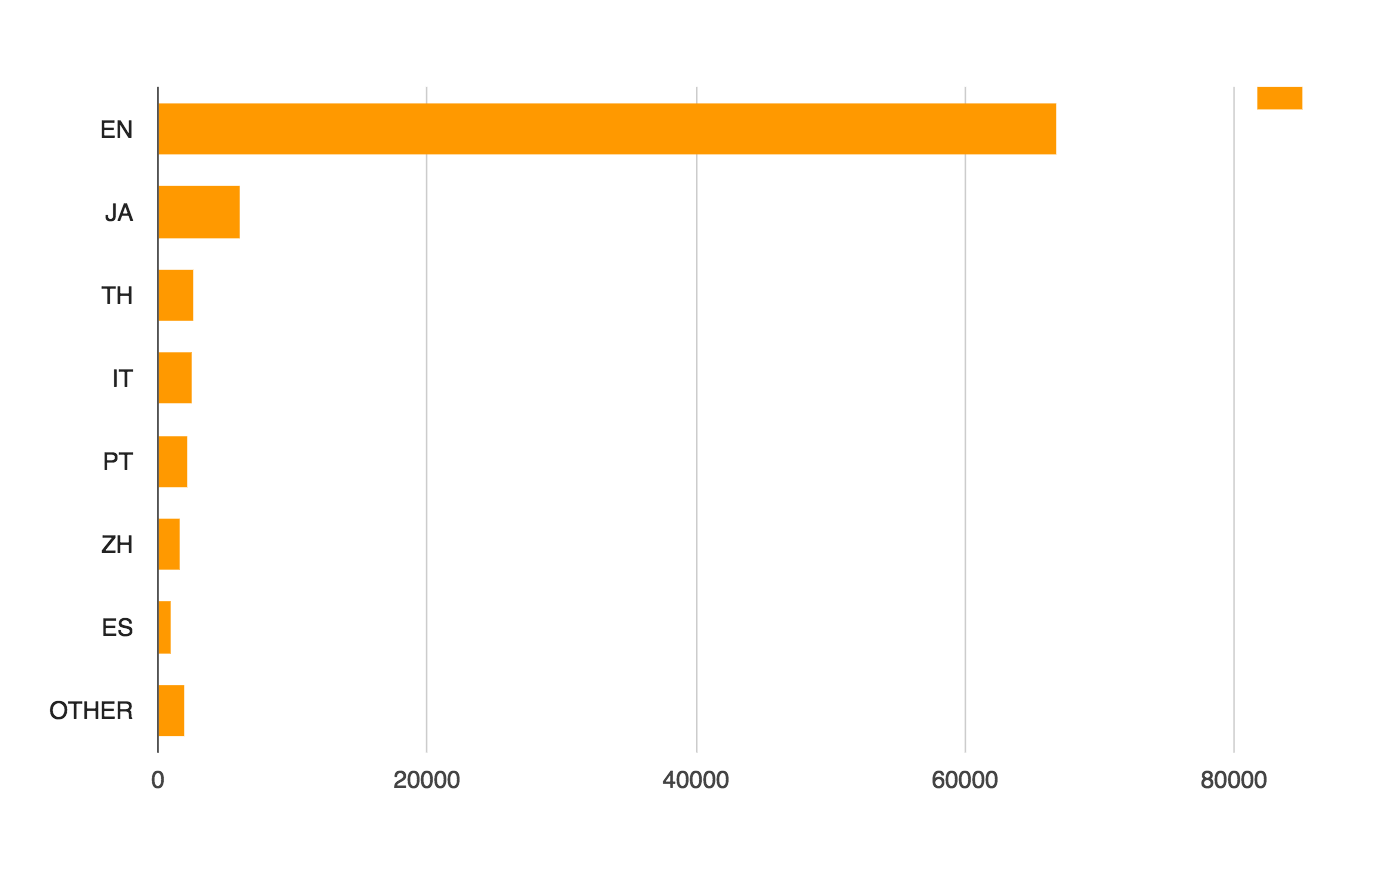
\includegraphics[width=400pt]{langs}.
 \caption{Language distribution in June 2013 data dump.}
 \label{figure:langs}
\end{figure}

For these languages, it might be wortwhile to set up a full syntactic processing chain, as they are all covered in Universal Dependencies. Indeed, for languages where we have few documents, frequency-based methods or ft-idf term extraction can be unrealiable, so relevant word associations obtained from dependency parsing could be an interesting information source.


\section{Conclusion}

My analysis is centered on messages marked as headlines or full articles, and does not include messages with the Alert event type, which are capitalized trading and stock-market messages. They belong to their own domain and have linguistic properties of their own, but one could conceivable also apply the tf-idf headline method described in Section \ref{sec:tfidf}.


\bibliography{biblio}
\bibliographystyle{unsrt}
%\bibliographystyle{bibliostyle}
\end{document}
                       
                       
  
  
  
  
  
  
  
  
  
  




\end{document}